\documentclass[12pt]{exam}
%\documentclass[12pt]{article}
\usepackage[letterpaper, margin=0.75in]{geometry}
\usepackage{graphicx}
\usepackage{enumitem}
\usepackage{booktabs}
\usepackage{amsmath}
\usepackage{tabularx}
\usepackage{color}
\usepackage{textcomp}

\begin{document}
\footer{}{Page \thepage\ of \numpages}{}

\begin{flushright}
\makebox[0.5\textwidth]{\large Name:\enspace\hrulefill}
\vspace{0.2in}

\makebox[0.5\textwidth]{\large Date:\enspace\hrulefill}
\end{flushright}

\begin{center}

\includegraphics[width=10cm]{../images/logo.png}
\end{center}

\begin{center}
\noindent{\LARGE Conceptual Physics \\ Class 7 Questions \\ March 23, 2018 \\ ~ \\ Practice Questions for First Partial Test \\}
\end{center}
\vspace{0.2in}

\clearpage
\begin{questions}

\question What is an ideology? What are scientific theories?
	\fillwithlines{2in}	
	
\question
Some philosophers assert that there is no difference between science and myth, and that modern science fills the same role as ancient myth, with no difference in its methods. What do you think? In what ways are modern science and ancient mythology similar and/or different?
\fillwithlines{3in}

\question
	Convert the following to centimeters (cm). Some useful conversion factors: 1~mile = 1.6~km, 1~light-year = $9\times 10^{15}~m$.
	\begin{parts}
		\part 15~m
			\vspace{0.5in}
		\part 10~miles
			\vspace{0.5in}
		\part 2~light-years
			\vspace{0.5in}
	\end{parts}

\clearpage
\question
You are an astronaut on Mars, passing the time by juggling. You are taking advantage of the fact that the acceleration due to gravity on the surface of Mars is only about 4 m/s$^2$, which allows you to have slower reaction times. You throw a ball straight upwards at 8 m/s.
\begin{parts}
\part Draw a sketch of the problem.
\vspace{3in}
\part How long does the ball take to reach the top of its trajectory?
\vspace{1.5in}
\part How high does the ball go?
\vspace{1.5in}
\part How long does the ball take to land back in your hand, from the moment you threw it?
\vspace{1.5in}
\end{parts}

\clearpage
\question
The following velocity \textit{vs.} time plot describes the random motion of someone running back and forth on a sidewalk. Let the positive direction indicate East, and negative direction be West.

\begin{center}
\noindent 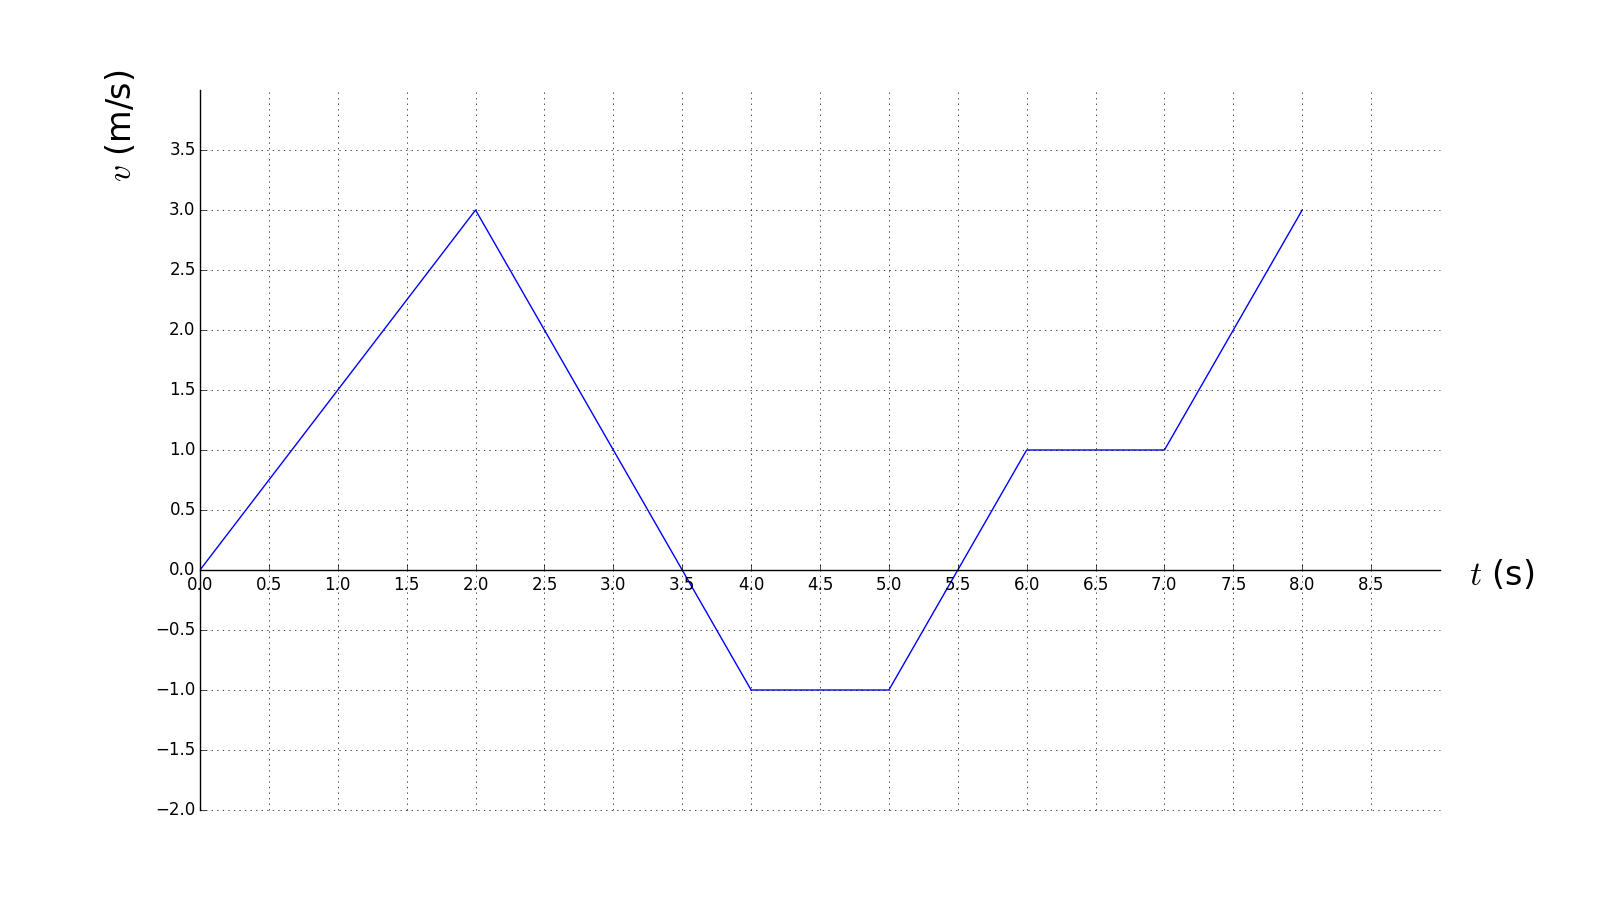
\includegraphics[width=0.9\textwidth]{../images/practtest1_plot.png}
\end{center}

\begin{parts}
\part When were they moving fastest?
\vspace{0.5in}
\part What was their greatest velocity?
\vspace{0.5in}
\part When were they not moving?
\vspace{0.5in}
\part When was their acceleration zero?
\vspace{0.5in}
\part When was their acceleration negative?
\vspace{0.5in}
\end{parts}

\clearpage
\question
Despite a very strong wind, a tennis player manages to hit a tennis ball with her racquet so that the ball passes over the net and lands in her opponent's court. Consider the following forces:
\begin{enumerate}
\item A downward force of gravity
\item A force by the ``hit''
\item A force exerted by the air
\end{enumerate}
Which of the above forces is (are) acting on the tennis ball after it has left contact with the racquet and before it touches the ground?
\begin{choices}
\choice 1 only
\choice 1 and 2
\choice 1 and 3
\choice 2 and 3
\choice 1, 2, and 3
\end{choices}

\question
The figure depicts a hockey puck sliding with a constant speed $v_0$ from point $a$ to point $b$ on a frictionless horizontal surface. Forces exerted by the air are negligible. You are looking down on the puck. When the puck reaches point $b$, it receives a swift horizontal kick in the direction of the heavy print arrow.
\begin{center}
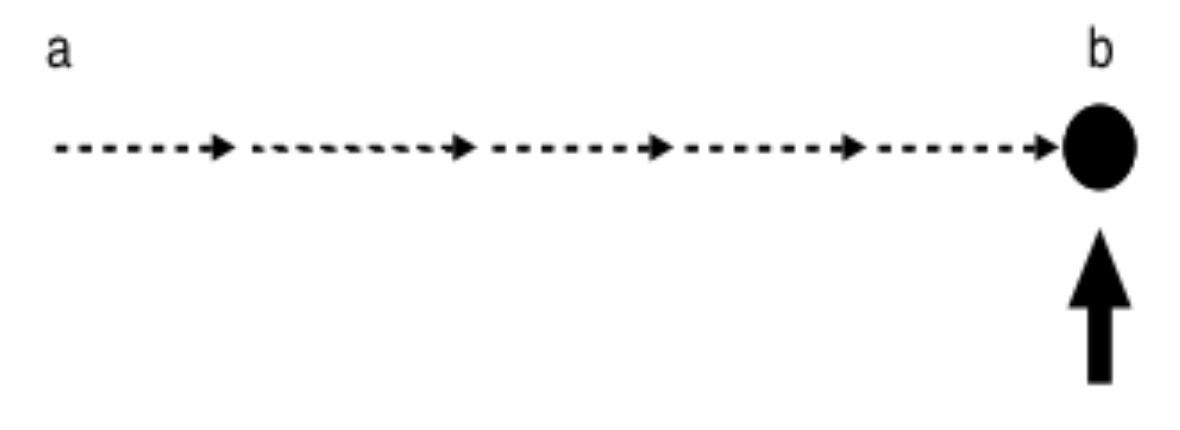
\includegraphics[width=0.8\textwidth]{../images/FCI_puck1.png}
\end{center}
\begin{parts}
\part
Which of the paths below would the puck most closely follow after receiving the kick?

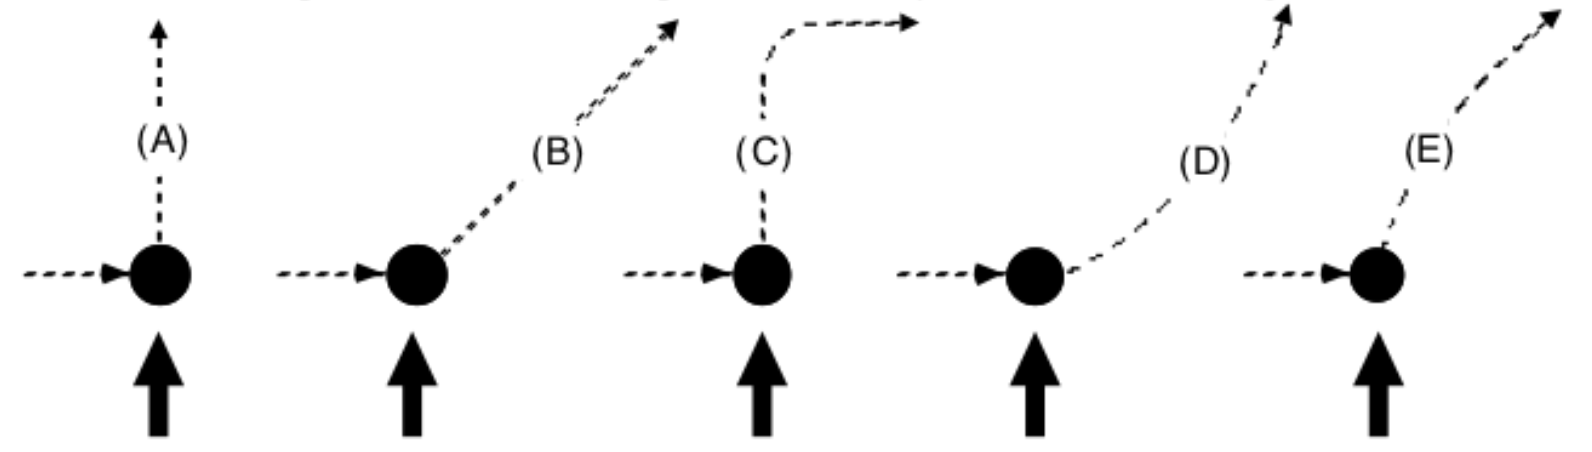
\includegraphics[width=0.8\textwidth]{../images/FCI_puck2.png}

\clearpage
\part
Along the frictionless path you have chosen above, the speed of the puck after receiving the kick:
\begin{choices}
\choice is constant.
\choice continuously increases.
\choice continuously decreases.
\choice increases for a while and decreases thereafter.
\choice is constant for a while and decreases thereafter.
\end{choices}

\part
Along the frictionless path you have chosen above, the main force(s) acting on the puck after receiving the kick is (are):
\begin{choices}
\choice a downward force of gravity.
\choice a downward force of gravity, and a horizontal force in the direction of motion.
\choice a downward force of gravity, an upward force exerted by the surface, and a horizontal force in the direction of motion.
\choice a downward force of gravity and an upward force exerted by the surface.
\choice none. (No forces act on the puck.)
\end{choices}
\end{parts}

\question
You are hiking on a glacier and come across a crevasse. It is too narrow for you to see the bottom, but you want to know how deep it is, so you drop a rock straight down ($v_0 = 0$~m/s) and listen for a splash, which you hear 2.0 s later. (For simplicity, assume the acceleration due to gravity is 10 m/s$^2$ downwards.)
\begin{parts}
\part Draw a sketch of the problem.
\vspace{3in}
\part What was the rock's velocity when it hit the bottom?
\vspace{1.5in}
\part What was the rock's average velocity during the fall?
\vspace{1.5in}
\part How deep is the crevasse?
\vspace{1.5in}
\end{parts}

\clearpage
\question
The following position \textit{vs.} time plot describes the motion of a toy train being pushed along a straight track, where $x=0$ is the center of the track and points to the right are positive. For questions that ask you to list points, \textbf{refer only to the labeled points.}

\begin{center}
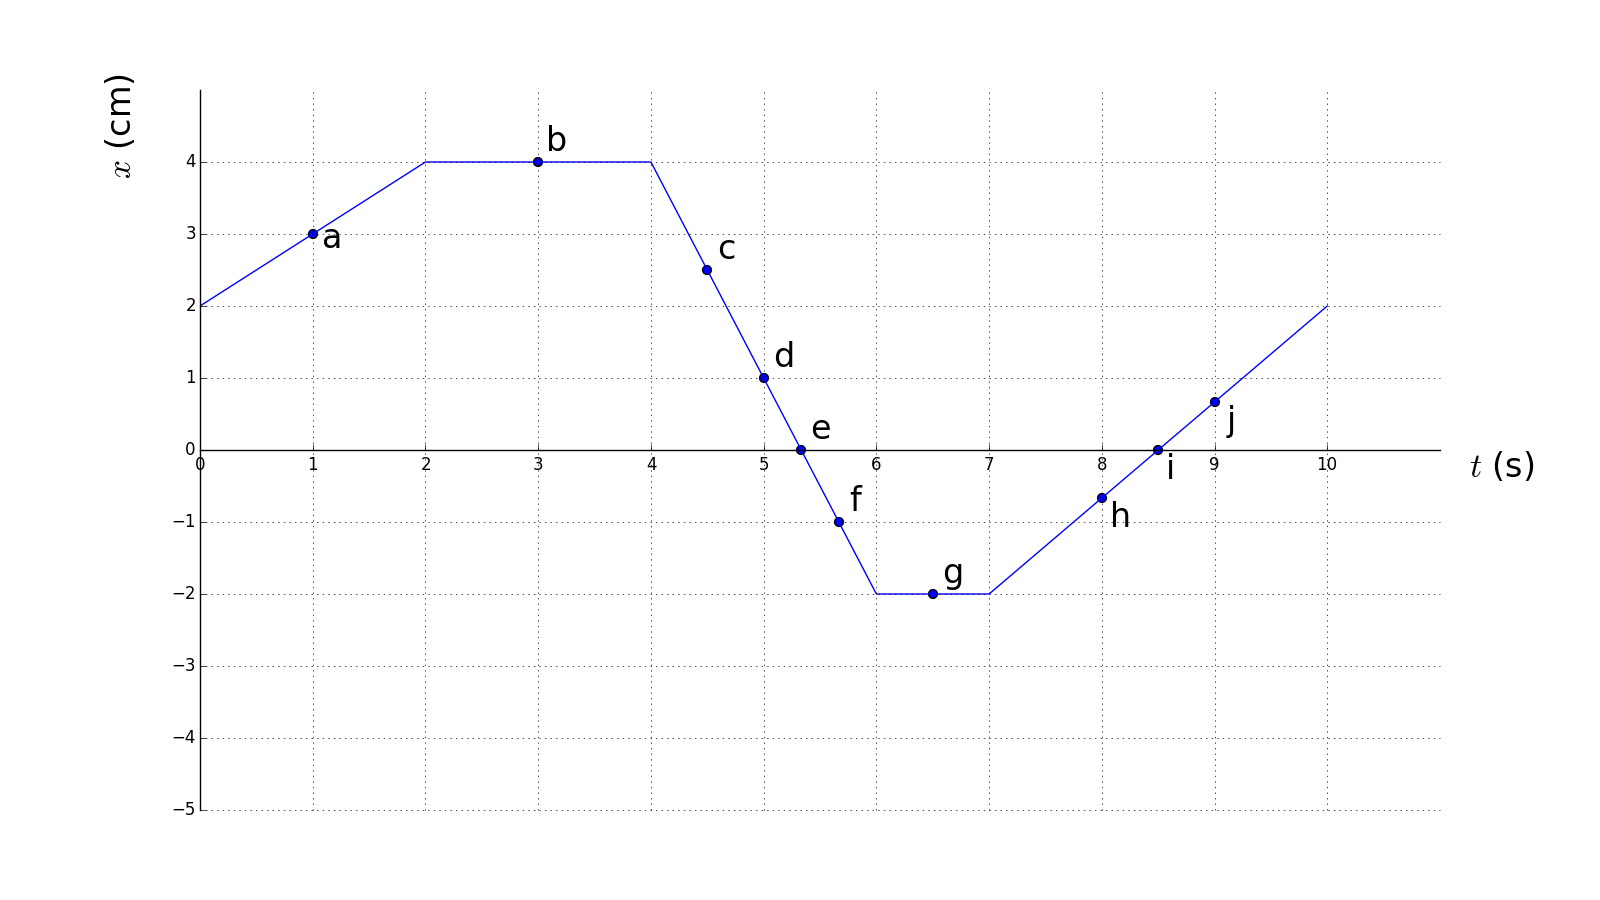
\includegraphics[width=\textwidth]{../images/test1_plot.png}
\end{center}

\begin{parts}
\part At which point(s) is the train not moving?
\vspace{0.5in}
\part At which point(s) is the train moving fastest?
\vspace{0.5in}
\part At which point(s) is the train farthest to the left?
\vspace{0.5in}
\part At which point(s) is the train \textit{moving} to the left?
\vspace{0.5in}
\part At which point(s) does the train experience zero acceleration?
\vspace{0.5in}
\part What is the train's displacement from $t=0$ to $t=10$~s?
\vspace{0.5in}
\end{parts}

\question
A boy throws a steel ball straight up. Consider the motion of the ball only after it has left the boy's hand but before it touches the ground, and assume that forces exerted by the air are negligible. For these conditions, the force(s) acting on the ball is (are):
\begin{choices}
\choice a downward force of gravity along with a steadily decreasing upward force.
\choice a steadily decreasing upward force from the moment it leaves the boy's hand until it reaches its highest point; on the way down there is a steadily increasing downward force of gravity as the object gets closer to the earth.
\choice an almost constant downward force of gravity along with an upward force that steadily decreases until the ball reaches its highest point; on the way down there is only a constant downward force of gravity.
\choice an almost constant downward force of gravity only.
\choice none of the above. The ball falls back to the ground because of its natural tendency to rest on the surface of the earth.
\end{choices}
\question
\label{ques:25}
A woman exerts a constant horizontal force on a large box. As a result, the box moves across a horizontal floor at a constant speed $v_0$.

The constant horizontal force applied by the woman:
\begin{choices}
\choice has the same magnitude as the weight of the box.
\choice is greater than the weight of the box.
\choice has the same magnitude as the total force which resists the motion of the box.
\choice is greater than the total force which resists the motion of the box.
\choice is greater than either the weight of the box or the total force which resists its motion.
\end{choices}

\question
If the woman in the previous question doubles the constant horizontal force that she exerts on the box to push it on the same horizontal floor, the box then moves:
\begin{choices}
\choice with a constant speed that is double the speed $v_0$ in the previous question.
\choice with a constant speed that is greater than the speed $v_0$ in the previous question, but not necessarily twice as great.
\choice for a while with a speed that is constant and greater than the speed $v_0$ in the previous question, then with a speed that increases thereafter.
\choice for a while with an increasing speed, then with a constant speed thereafter.
\choice with a continuously increasing speed.
\end{choices}

\question
If the woman in question~\ref{ques:25} suddenly stops applying a horizontal force to the box, then the box will:
\begin{choices}
\choice immediately come to a stop.
\choice continue moving at a constant speed for a while and then slow to a stop.
\choice immediately start slowing to a stop.
\choice continue at a constant speed.
\choice increase its speed for a while and then start slowing to a stop.
\end{choices}

\clearpage
\question Consider 2 planets, planet $A$ and planet $B$, orbiting a distant star. The following 3 scenarios have the two planets located at different distances and with varying masses, and will ask you to compare the gravitational forces experienced by them.
\begin{parts}
	\part Planet $A$ and planet $B$ are identical, and orbit the star at different distances. Planet $A$ is \textbf{twice as far away} from the star as planet $B$. Which, if any, experiences the greater gravitational attraction to the star? Why?
	\begin{center}
	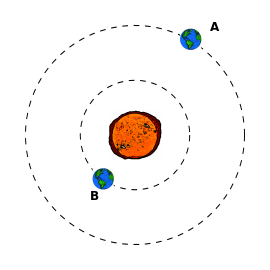
\includegraphics{../images/2PlanetsA.png}
	\end{center}
	
	\clearpage
	\part Planet $A$ has \textbf{twice the mass} of planet $B$, and they are orbiting at the same distance from the star. Which, if any, experiences the greater gravitational attraction to the star? Why?
	\begin{center}
	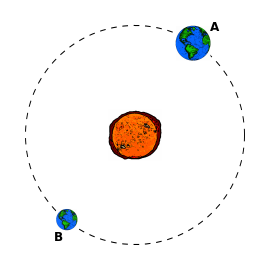
\includegraphics{../images/2PlanetsB.png}
	\end{center}
	
	\part Planet $A$ is located \textbf{twice as far away} as planet $B$, but \textit{also} has \textbf{twice the mass} as planet $B$. Which, if any, experiences the greater gravitational attraction to the star? Why?
	\begin{center}
	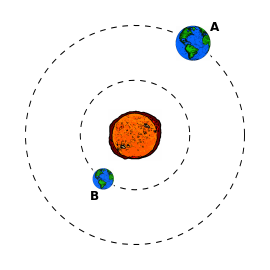
\includegraphics{../images/2PlanetsC.png}
	\end{center}
	
	\end{parts}

\clearpage
\question The Earth's orbit around the Sun is not perfectly circular. Below is a (highly exaggerated) schematic of the Earth's elliptical orbit. Assume that energy is conserved in the Earth+Sun system.
\begin{center}
	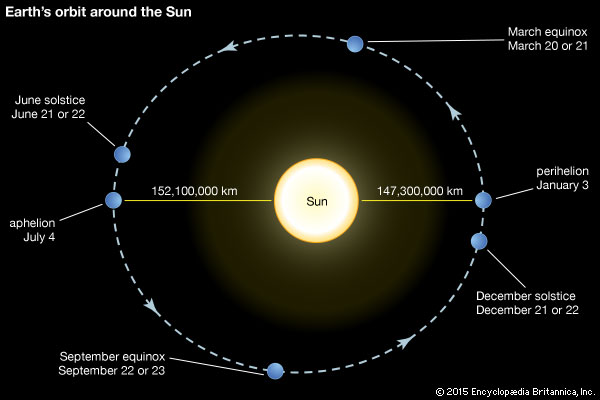
\includegraphics[width=0.7\textwidth]{../images/test2_seasons.jpg}
	\end{center}
	\begin{parts}
	\part When is the Earth moving the fastest around the Sun? When is it moving the slowest?
	\vspace{1in}
	\part When does the Sun do positive work on the Earth? Negative work? Zero work?
	\vspace{1.5in}
	\end{parts}

\question You are an astronaut looking for a new planet that reminds you of home.
\begin{parts}
\part You find a planet with three times the mass of Earth's and the same radius. How would the gravitational force on you on the surface of the planet compare to the gravitational force on you on the surface of the Earth?
\vspace{1in}
\part You find a planet with the same mass as Earth and one half the radius. How would the gravitational force on you on the surface of the planet compare to the gravitational force on you on the surface of the Earth?
\vspace{1in}
\part You find a planet with four times the mass of Earth and twice the radius. How would the gravitational force on you on the surface of the planet compare to the gravitational force on you on the surface of the Earth?
\vspace{1in}
\end{parts}

\question Explain, using the properties of the electrostatic (Coulomb) force and the strong nuclear force, why all of the heaviest elements (elements with the most protons and neutrons in the nucleus) are unstable. Feel free to draw diagrams that help your explanation.
\vspace{3.5in}

\clearpage
\question You are attempting to move a 20-kg cardboard box across a room and then upstairs. For each stage, describe the \textbf{change} in the box's energy, and say whether \textbf{you} did positive, negative, or zero work on the box. (For this problem, you can ignore the effects of air resistance but friction between the box and the floor is \textbf{not} negligible.)
\begin{center}
	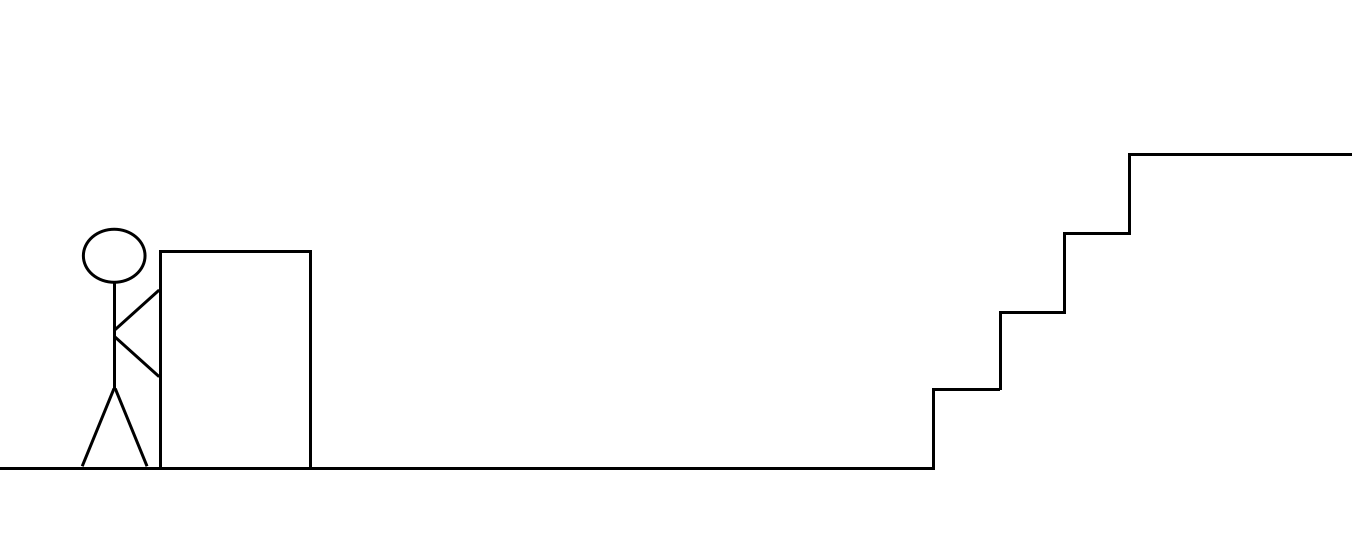
\includegraphics[width=0.7\textwidth]{../images/test2_stairs.png}
	\end{center}
\begin{parts}
\part You apply a horizontal force to the box as you accelerate from rest to 1 m/s in 1 s.
\vspace{0.5in}
\part You push the box at a constant velocity of 1 m/s for 5 s.
\vspace{0.5in}
\part You stop pushing the box and allow it to come to rest in 1 s.
\vspace{0.5in}
\part You lift the box to a height of 1 m.
\vspace{0.5in}
\part Holding the box at a constant height, you accelerate from rest to 1 m/s in 2 s.
\vspace{0.5in}
\part You carry the box up a 3 meter flight of stairs at a constant speed of 1 m/s.
\vspace{0.5in}
\part You continue to carry the box at a constant height and a constant velocity of 1 m/s for 5 s.
\vspace{0.5in}
\part Holding the box at a constant height, you slow to a stop in 1 s.
\vspace{0.5in}
\end{parts}

	
	\question
	What is the difference between \textbf{displacement} and \textbf{distance}? Describe a situation in which an object travels a nonzero distance, yet experiences zero displacement.
	\vspace{1in}
	
	\question
	What is the difference between \textbf{speed} and \textbf{velocity}? Describe a situation in which an object's speed is constant, but its velocity is changing.
	\vspace{1in}

	
	\question \textit{Particle accelerators}, as the name implies, are used to accelerate particles. These are used in a variety of experiments, such as colliders which smash particles together to better understand fundamental physics.
	
	Particles are not always accelerated at a constant rate, but rather experience ``acceleration bursts". The graph below shows the acceleration of a particle, as a function of time. There are 3 different ``acceleration bursts", (1) from 0~s~to~5~s, (2) from 6~s~to~11~s, and (3) 12~s~to~17~s.
	
	\begin{center}
	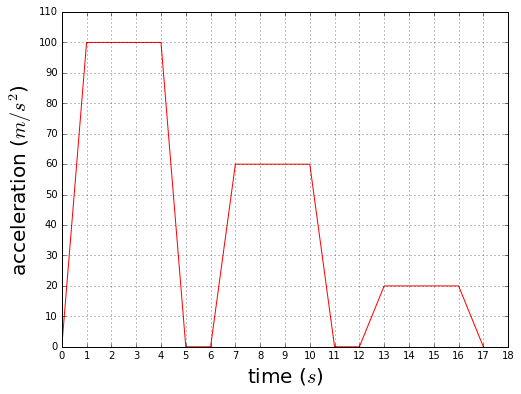
\includegraphics[width=4in]{../images/accelBursts.png}
	\end{center}
	
	\begin{parts}
		\part During which burst (1, 2 or 3) does the particle experience the \textbf{greatest change in velocity}? Please explain your answer.
			\vspace{1in}
			\clearpage
		\part Describe the particle's motion from t=5~s to t=6~s.
			\vspace{1in}
		\part Assuming the particle begins at rest, when does the particle have the \textbf{greatest velocity}? What is this maximum velocity?
		\vspace{1in}
	\end{parts}

	\question
	Cars are designed with ``crumple zones", to reduce the impact of a collision on passengers. A person driving in winter skids on ice and collides their vehicle head on with a post. If they were initially traveling at 10~m/s, and during the crash the front compartment of their car crumples 1~m to absorb some of the impact, then:
	\begin{parts}
	\part What is the acceleration experienced by the driver in units of $m/s^2$? (\textbf{assume constant acceleration})
		\vspace{2in}
	\part What is the acceleration experienced by the driver in units of $g = -10~m/s^2$?
		\vspace{2in}
	\part In order for the driver to experience an acceleration of $1.8~g$, what would their initial velocity need to be, assuming the car still crumpled by 1~m?
		\vspace{2in}
	\end{parts}
	
\question Two objects, each with mass $m$ and a positive charge $q$, are pushed towards each other with some velocity. The following 2 images show the two as they approach each other. Image $1$ represents their initial locations, where they are a distance $2r$ apart. Image $2$ shows their final positions, where they are a smaller distance $r$ apart. Use these images to answer the following questions.
\vspace{0.1in}
\begin{center}
\input{../images/2massCharges.pdf_tex}
\end{center}
\vspace{0.1in}
\begin{parts}
	\part Is it possible to tell how the electric force between them changes? If so, does it increase, decrease or stay the same?
		\vspace{1in}
	\part Is it possible to tell how the electric potential energy changes? If so, does it increase, decrease or stay the same?
		\vspace{1in}
	\part Is it possible to tell how the gravitational force between them changes? If so, does it increase, decrease or stay the same?
		\vspace{1in}
	\part Is it possible to tell how the gravitational potential energy changes? If so, does it increase, decrease or stay the same?
		\vspace{1in}
\end{parts}

\end{questions}

\end{document}
